%===================================================================================================
\subsection{Approach}\label{mod.cal.appr}
We used an adapted version of the
Incremental Mixture Importance Sampling (IMIS) procedure \cite{Raftery2010} for model calibration.
% TODO
%---------------------------------------------------------------------------------------------------
\subsubsection{Sampling with Relational Constraints}\label{mod.cal.appr.jsam}
We imposed the following relational constraints on calibrated parameter values during sampling:
\begin{itemize}\singlespacing
  \item[a.] \texttt{K_swo_fsw_h * F_swo + K_swr_fsw_h * F_swr < 2*365}\\
  where: \texttt{K_swx_fsw_h = C1m_swx_fsw_h * dur_swx / (dur_swx + 1/12)}
  \item[b.] Let ``\texttt{c_}'' denote \texttt{PF_condom_}:\\
  \texttt{c_msp_2006 < c_msp_2016}\\
  \texttt{c_cas_2006 < c_cas_2016}\\
  \texttt{c_swo_2002 < c_swo_2011 < c_swo_2014}\\
  \texttt{c_swr_2002 < c_swr_2011 < c_swr_2014}\\
  \texttt{c_msp_2006 < c_cas_2006}\\
  \texttt{c_msp_2016 < c_cas_2016}\\
  \texttt{c_swr_2002 < c_swo_2002}\\
  \texttt{c_swr_2011 < c_swo_2011}\\
  \texttt{c_swr_2014 < c_swo_2014}
  \item[c.] \texttt{1 <= (Rbeta_acute * dur_acute) <= 63}
  \item[d.] \texttt{P_gud_fsw_l > .07}\\
  \texttt{(P_gud_fsw_l * RP_gud_fsw_h:l) < 1}
\end{itemize}
For each set of constraints, parameters were repeatedly sampled until all constraints were satisfied.
As shown in Figure~\ref{fig:jsam.bias},
this approach reduces distortion of sampled \vs prior distributions,
as compared to forward/backward conditional sampling.
Constrained parameters were therefore omitted from initial Latin hypercube sampling.
\begin{figure}[h]
  \centering
  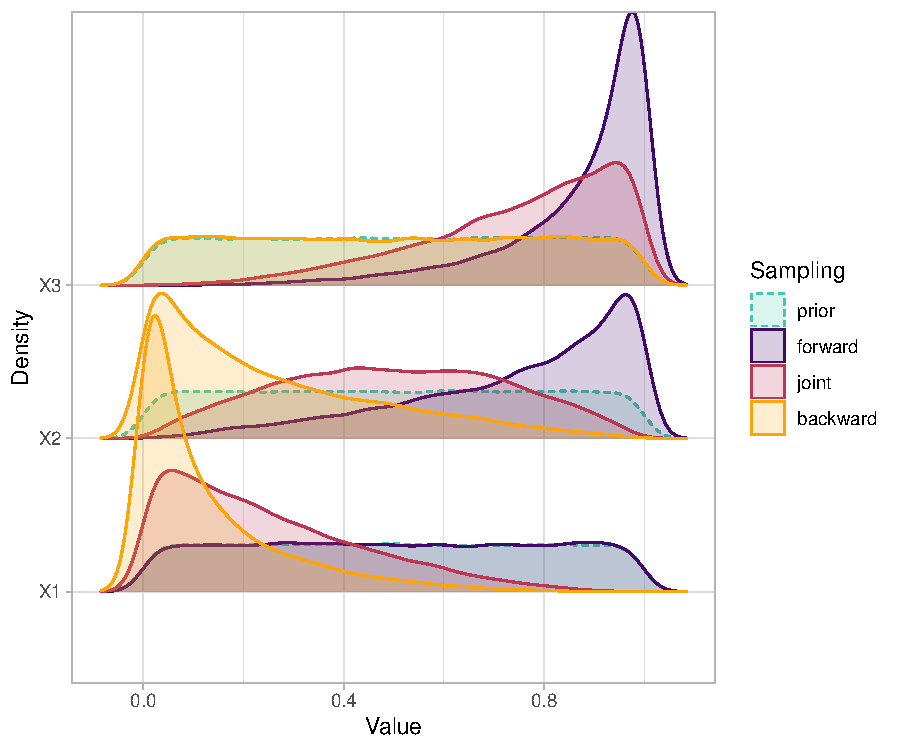
\includegraphics[width=.6\linewidth]{jsam.bias}
  \caption{Illustration of different sampling biases when enforcing $X_1 < X_2 < X_3$}
  \label{fig:jsam.bias}
  \floatfoot{Sampling method:
    \emph{joint:} sample $X_1$, $X_2$, $X_3$ simultaneously; then discard any samples failing $X_1 < X_2 < X_3$;
    \emph{forward:} sample $X_1$; then sample $X_2$ until $X_1 < X_2$; then sample $X_3$ until $X_2 < X_3$;
    \emph{backward:} sample $X_3$; then sample $X_2$ until $X_2 < X_3$; then sample $X_1$ until $X_1 < X_2$.}
\end{figure}
